\begin{tikzpicture}
\node [mybox] (box){%
    \begin{minipage}{0.3\textwidth}
        \txt{
        Mat vertical de 2m de hauteur est fixé au fond d'une piscine et dépasse la surface de l'eau de 0.5m. Le soleil se trouve à 45deg. au dessus de l'horizon. \textbf{Longueur de l'ombre au fond de la piscine?}
        
        % 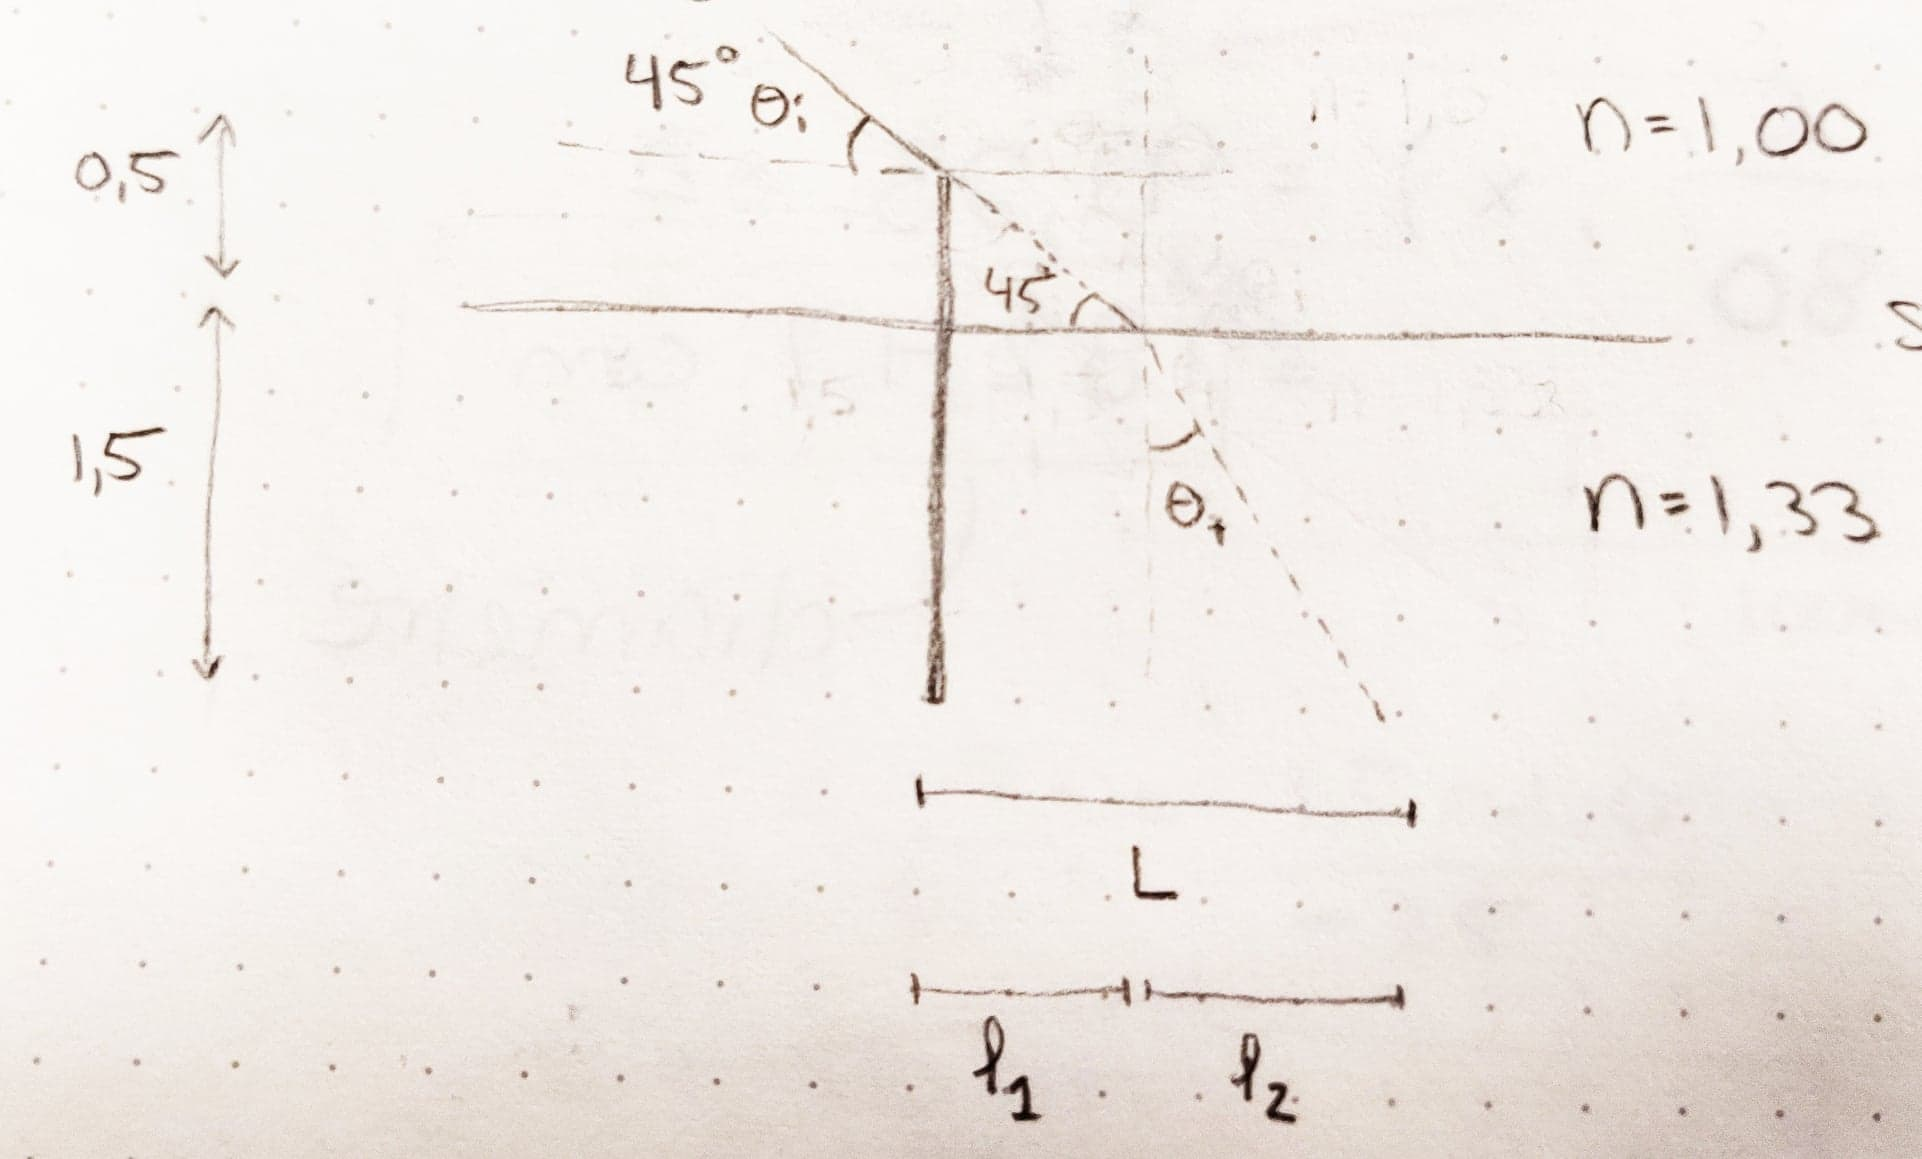
\includegraphics[scale=0.05]{images/graph_ex_refraction.jpg}
        
        \begin{equation*}
        solve = \begin{cases}
            tan(45^\circ) = \frac{0.5}{L_1}\\
            1.00\ sin(45^\circ) = 1.33\ sin(\theta_t) \\
            tan(\theta_t) = \frac{L_2}{1.5}
        \end{cases}
        |\ 0 < \theta_t < 180
        \end{equation*}
        }
        $$\theta_t=32.12^\circ,\ L_1=0.5m,\ L_2=-0.94m$$
        $$|L_1| + |L_2| = 1.44m$$
    \end{minipage}
};
% \node[fancytitle, right=10pt] at (box.north west) {Exercice réfraction};
\end{tikzpicture}